\subsection{Generalized Brent's theorem}

In order to relate the total work and total depth of a program with
its execution time, we rely on Brent's theorem. This theorem is
usually formulated in terms of {\em computation DAGs}. 
%
%
%In what follows, we recall the traditional statement of Brent's
%theorem, and adapt it to our cost semantics.
%
%TODO:  Brent's theorem. assumes a greedy scheduler that can perform 
%load balancing without overheads. 
%
A computation DAG is a directed acyclic graph that represents a
parallel computation. Nodes in the graph represent atomic
computations.  Edges between nodes represent precedence relations, in
the sense that an edge from $a$ to $b$ indicates that the execution of
$a$ must be completed before the execution of $b$ can start.  Every
computation DAG includes a {\em source} node and a {\em sink} node,
representing the starting and the end points of the computation,
respectively.  Those nodes are such that all nodes of a computation
DAG are reachable from the source node, and the sink node is reachable
from all nodes.  An example computation DAG appears in \figref{dag}.
A node is said to be {\em ready} if all the nodes that points to it
have already been executed.

Brent's theorem gives a bound on the time required for executing all
the tasks in a computation DAG with a greedy scheduler, assuming that
each node takes a unit of time to execute. A scheduler is said to be
{\em greedy} if it never stays idle unnecessarily, i.e., when there
exists a ready node the scheduler finds it at no cost and executes
it.  Typical proofs of Brent's theorem assume a unit cost model where
each instruction costs a unit cost to execute and construct a
``level-by-level'' execution schedule.  


One way to extend the Brent's theorem to include task-creation
overheads is to assign a weight to each node. Proving such a
generalization directly, however, turns out to be highly nontrivial
and in our attempts resulted in relatively complex proofs.  Another
approach is to represent non-unit cost tasks with a sequence of unit
tasks, e.g., we can replace a task with weight three with a sequence
of three unit-cost tasks.  Since overheads are non-divisible work, we
would require that such tasks execute on the same processors back to
back without interleaving with other tasks.  With this approach,
typical proofs of Brent's theorem, which assume a ``level-by-level''
execution schedule, do not work because they break up
sequences. Fortunately, we have found that Arora et al's
proof~\cite{AroraBlPl98} can be adapted easily for this purpose,
because it makes no assumption about ordering of ready nodes, directly
allowing us to generalize Brent's theorem to include task-creation
overheads.

 

\begin{figure}
\centering
\ifx\arthur\false
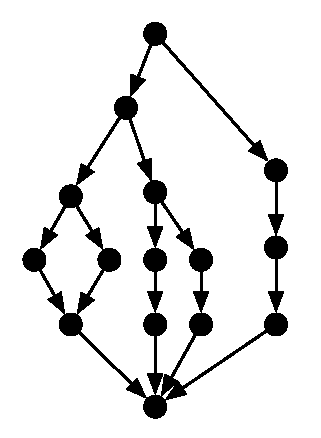
\includegraphics[width=0.4\columnwidth]{pictures/computation-dag}
\fi
\caption{An example computation DAG.}
\label{fig:dag}
\end{figure}



\begin{theorem}[Brent's theorem for computation DAGs]
\label{thm:basic-brent}
Let $G$ be a computation DAG made of $W$ nodes and whose
longest path has length $D$.
%Let $W$ be the number of nodes in $G$ and $D$ be the length of
%the longest path in $G$.
Any greedy scheduler can 
execute this computation DAG in no more than $\frac{W}{P} + D$ 
steps on $P$ processors. 
\end{theorem}
\begin{proof}
At each execution step, each processor places a token in the {\em work bucket}
if it is busy at this step, otherwise it places a token in the {\em idle bucket}.
The work bucket contains exactly $W$ tokens at the end of the execution.
Let $I$ be the number of tokens contained in the idle bucket at the end of the
execution, and let $T$ denote the total number of steps in the execution.
Because a total $T P$ tokens are created, we have $T P = W + I$.
In order to establish the result $T \leq \frac{W}{P} + D$,
it thus suffices to establish the inequality $I \leq P D$.

Consider a given time step.
If all processors are executing then the idle bucket
receives zero tokens. Otherwise, a number of processors are idle.
In this case, the idle bucket receives between one and $P-1$ tokens.
We can bound the number of time steps at which this situation happens,
as follows. 
If one or more processors are idle, it means that those processors cannot
find a ready task to execute. Because the scheduler is assumed to be greedy,
it must be the case that all the ready tasks are currently executing.
Therefore, at such a time step, the maximal length of a path 
in the computation DAG starting from a ready node decreases by one unit. 
Because the maximal length of a path in the computation DAG is initially $D$,
there can be at most $D$ time steps at which not all processors are executing.
It follows that the final number of tokens in the idle bucket
does not exceeed $(P-1) D$. This result entails the inequality $I \leq P D$. \qed
\end{proof}

Observe that the proof does not impose any constraint on the order in
which the ready tasks should be executed by the processors.  So, if one
processor starts working on a sequence of several nodes, then it can
execute all the nodes in the sequence before looking for other ready
tasks.  Therefore, the proof accepts computation DAGs that encode
non-unit tasks as sequences of unit tasks.  We will make use of such
an encoding in the proof of our next theorem, which relates our cost
semantics to the computation DAG model.  

%% We consider here the case of the oracle semantics, for which we encode
%% the costs $\csp$ and $\corc$ by placing additional nodes in the DAG,
%% but a similar construction could be applied for the other evaluation
%% modes.

\begin{theorem}[Brent's theorem for the cost semantics] 
\label{thm:generalize-brent}
\label{thm:generalized-brent}~\\
%Let $e$ be an expression whose total work is $\sws$ and whose total 
%depth is $\sds$. In other words, 
Assume 
$\Jcostof{\sorc}{ e }{ v }{\sw}{\sd}{\sws}{\sds}$
to hold for some $v$, $\sw$ and $\sd$.
Any greedy scheduler can execute the expression $e$
in no more than $\frac{\sws}{P} + \sds$ computations steps on $P$ processors. 
\end{theorem}
\begin{proof}
In order to invoke the version of Brent's theorem that applies 
to computation DAGs, we build the computation DAG associated 
with the execution of the expression $e$, including nodes that
represent the cost of scheduling.
To that end, we describe a recursive algorithm for turning 
an expression $e$ with total work $\sws$ and total depth $\sds$
into a corresponding computation DAG containing $\sws$ nodes and
whose longest path has length $\sds$.
The algorithm follows the structure of the derivation that
$e$ has total work $\sws$ and total depth~$\sds$.
\begin{itemize}
\item If the last rule has zero premises, then $e$ is an atomic expression
and $\sws = \sds = 1$. We build the corresponding DAG as a single node.
\item If the last rule has one premise, then $\sws$ takes the form $\sws_1 + 1$
and $\sds$ takes the form $\sds_1 + 1$. Let $G_1$ be the DAG corresponding
to the sub-expression described in the premise. We build $G$ by 
extending $G_1$ with one node at the bottom, that is, by
sequentially composing $G_1$ with a DAG made of a single node. 
\item Otherwise the last rule has two premises.
First, consider the case where $e$ is a let-expression. 
$\sws$ takes the form $\sws_1 + \sws_2 + 1$
and $\sds$ takes the form $\sds_1 + \sds_2 + 1$.
Let $G_1$ and $G_2$ be the DAGs corresponding to the two sub-expressions.
We build $G$ by sequentially composing $G_1$ with a single node and then 
with $G_2$.
\item Consider now the case of a parallel tuple that is sequentialized.
$\sws$ takes the form $\sws_1 + \sws_2 + 1 + \corc$
and $\sds$ takes the form $\sds_1 + \sds_2 + 1 + \corc$.
Let $G_1$ and $G_2$ be the DAGs corresponding to the two branches.
We build $G$ by sequentially composing $1 + \corc$ unit-cost nodes
with the sequential composition of $G_1$ and $G_2$.
\item Finally, consider the case of a parallel tuple that is parallelized.
$\sws$ takes the form $\sws_1 + \sws_2 + 1 + \csp + \corc$
and $\sds$ takes the form $\kwmax{\sds_1}{\sds_2} + 1 + \csp + \corc$.
Let $G_1$ and $G_2$ be the DAGs corresponding to the two branches.
We build $G$ by sequentially composing $1 + \csp + \corc$ unit-cost nodes
with the parallel composition of $G_1$ and $G_2$. 
\end{itemize}
It is straightforward to check that, in each case, $\sws$ and $\sds$ 
match the number of nodes and the total depth of the DAG being produced. \qed
\end{proof}
